\documentclass{school-22.101-notes}
\date{October 12, 2011}

\begin{document}
\maketitle

\subtopic{Case 1, $\ddt \expect{x}, \hat{H} = \frac{\hat{p}^2}{2m} + V(x) $}

\begin{align}
\ddt \expect{x} &= \frac{i}{\hbar} \expect{\left[ \hat{H}, \hat{x} \right]} \\
&= \frac{i}{\hbar} \expect{\left[ \frac{\hat{p}^2}{2m} + V(x), \hat{x} \right]} \\
&= \frac{i}{\hbar} \expect{\left[ \frac{\hat{p}^2}{2m} , \hat{x} \right]} \\
&= \frac{i}{2m\hbar} \expect{\left[ \hat{p}^2 , \hat{x} \right]} \\
&= \frac{i}{2m\hbar} (-2i\hbar \hat{p} ) \\
&= \boxed{\frac{1}{m} \expect{p} = \expect{v}}
\end{align}

\subtopic{Case 2, $\ddt \expect{p}, \hat{H} = \frac{\hat{p}^2}{2m} + V(x) $}

\begin{align}
\ddt \expect{p} &= \frac{i}{\hbar} \expect{\left[ \hat{H}, \hat{p} \right]} \\
&= \frac{i}{\hbar} \expect{\left[ \frac{\hat{p}^2}{2m} + V(x), \hat{p} \right]} \\
&= \frac{i}{\hbar} \expect{\left[ V(x) , \hat{p} \right]} \\
&= \frac{i}{\hbar} \expect{\left[ V(x), - i\hbar \ppx \right]} \\
&= \frac{i}{\hbar} \expect{(-i\hbar) (V(x) \ppx - \ppx V(x))} \\
&= \frac{i}{\hbar} \expect{i\hbar\pVpx} \\
&= \boxed{- \expect{\pVpx} = \expect{\mathrm{Force}} }
\end{align}
This is called Ehrenfest's Principle, which is a quantum mechanical equation for average/expectation values of p(t). 

\lecture{Angular Momentum}
Angular momentum is a conserved quantity in a central force field. While a general potential is dependent on the spatial coordinate:
\eqn{ V(\uline{x}) = V(r,\theta, \phi)   }
a special potential that is only depend on radius (no $\theta, \phi$ dependency) is called a central force field because of its rotational symmetry. 


\topic{Orbital Angular Momentum}
This is similar to its classical description of angular momentum. 

\subtopic{Construct Cartesian Components of $\hat{L}$}
We define the orbital angular momentum like:
\begin{align}
\hat{\uline{L}} &= \hat{\uline{r}} \cross \hat{\uline{p}} \\
\hat{\uline{L}}_x &= \hat{y} \hat{p}_z - \hat{z} \hat{p}_y = - i\hbar \left( y \ppz - z \ppy \right) \\
\hat{\uline{L}}_y &= \hat{z} \hat{p}_x - \hat{z} \hat{p}_x = - i\hbar \left( z \ppx - x \ppz \right) \\
\hat{\uline{L}}_z &= \hat{x} \hat{p}_y - \hat{y} \hat{p}_x = - i\hbar \left( x \ppy - y \ppx \right) 
\end{align}

\subtopic{Check the Components We Just Constructed}
The question we want to ask is, `can we find the eigenvalues of each of the operators simultaneously?'

To answer the above question, we consider whether the components commute with each other. Because if $\left[ \hat{L}_x, \hat{L}_y \right] = 0$, that is to say we can pin $L_x, L_y$ at the same time. 

Though when we derive it for real (see notes), they come out to be:
\eqn{ \left[ \hat{L}_x, \hat{L}_y \right] = i \hbar ( \hat{x} \hat{P}_y - \hat{y} \hat{P}_x) = i\hbar \hat{L}_z }
\eqn{ \left[ \hat{L}_y, \hat{L}_z \right] = i \hbar ( \hat{y} \hat{P}_z - \hat{z} \hat{P}_y) = i\hbar \hat{L}_x }
\eqn{ \left[ \hat{L}_z, \hat{L}_x \right] = i \hbar ( \hat{z} \hat{P}_x - \hat{x} \hat{P}_z) = i\hbar \hat{L}_y }

That is to say, $\hat{L}_x, \hat{L}_y, \hat{L}_z$ do not have common eigenstates, and that we cannot find $L_x, L_y, L_z$ simultaneously. 

\subtopic{Define the Orbital Angular Momentum Operator $\Lhat^2$}
What the above argument leads to is the $\hat{L}^2$,  a more physical term, and the square root of its eigenvalue is the angular momentum. 
\eqn{ \left[ \hat{L}^2, \hat{L}_x   \right] =  \left[ \hat{L}^2, \hat{L}_y   \right] =  \left[ \hat{L}^2, \hat{L}_z   \right] = 0   }
We can solve for the total angular momentum and the azimuthal component simultaneously in a coordinate system as illustrated in Figure~\ref{3DCS}. 
\begin{figure}
    \centering
    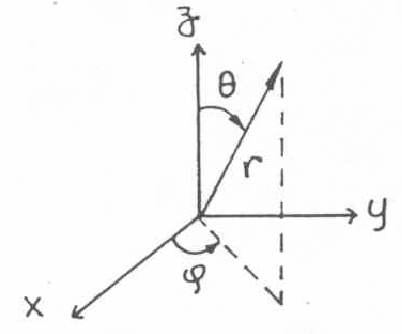
\includegraphics[width=2in]{images/qm/3DCS.png}
    \caption{Set-up of the 3D Coordinate System\label{3DCS}}
\end{figure}
\eqn{ \hat{L}_z = - i \hbar \ppphi }
\eqn{ \hat{L}^2 =  - \hbar^2 \left[ \frac{1}{\sin \theta} \pptheta \left( \sin \theta \pptheta \right) + \frac{1}{\sin^2 \theta} \ppphin2  \right] }

\subtopic{Define the Total Angular Momentum $\Jhat$}
We define the Total Angular Momentum as:
\eqn{ \Jhat = \Lhat + \Shat }
Notice we cannot solve for the three components of $\Jhat$ simultaneously neither, because: 
\eqn{ \left[ \Jhat_x, \Jhat_y \right] = i \hbar \Jhat_z,  \left[ \Jhat_y, \Jhat_z \right] = i \hbar \Jhat_x, \left[ \Jhat_z, \Jhat_x \right] = i \hbar \Jhat_y }


\subtopic{Eigenvalues of $\Lhat, \Jhat$}
See Liboff 9.3 for how we get the following equations: 
\eqn{ \boxed{ \hat{L}^2 \phi_{l,m} (\theta, \phi) = \hbar^2 l (l+1) \phi_{l,m} (\theta, \phi ), \fsp \fsp \hat{L}_z \phi_{l,m} (\theta, \phi) = \hbar m \phi_{l,m} (\theta, \phi ) } }
in which $l = 0,1,2, \cdots, m = -l, -l+1, \cdots, 0, \cdots l$. If we solve for $\hat{L}_x$ or $\hat{L}_y$ instead we will reach the same results as above. 

Similarly $\Jhat$ would give us:
\eqn{  \Jhat^2 \phi_{l,m} (\theta, \phi) = \hbar^2 j (j+1) \phi_{l,m} (\theta, \phi ), \fsp \fsp \Jhat_z \phi_{l,m} (\theta, \phi) = \hbar m_j \phi_{l,m} (\theta, \phi )  }
in which $j = 0,1/2,1,3/2,2, \cdots, m = -j, \cdots, j$. If we solve for $\Jhat_x$ or $\Jhat_y$ instead we will reach the same results as above. 

\subtopic{Eigenfunctions $\phi_{l,m}$ is Spherical Harmonics $Y_l^m(\theta, \phi)$}
The eigenfunction in the above equation, $\phi_{l,m}$, are commonly called the \textbf{Spherical Harmonics $Y_l^m (\theta, \phi)$}:
\eqn{ Y_l^m (\theta, \phi) = \frac{1}{\sqrt{2 \pi}} e^{im\phi} P_l^m (\phi)   }
A couple of things about the Spherical Harmonics:
\begin{itemize}
\item $\psi( r, \theta, \phi) = R(r) Y_{lm} (\theta, \phi)$. 
\item $\int_0^{2\pi} \dphi \int_0^{\pi} \sin \theta \dtheta |Y_{lm} (\theta, \phi) |^2 = 1.$
\item Spherical Harmonics also implies that the unit of angular momentum is $\hbar$.
\item Degeneracy: \textbf{For a given $l$ value, there are $2l+1$ number of degeneracy.} For instance, for $l=5$, we have 11 eigenstates $Y_5^5, Y_5^4, \cdots Y_5^{-5}$ that correspond to the same $l$, or the same $L^2 = 30 \hbar^2$. That is, for the same $L^2$, the projection onto the azimuthal plan are degenerate.  
\item $L_z$ is not continuous. Given a $L^2$, we can draw a bunch of cones, each surface describe the superposition of possible eigenfunctions. L will never entirely align with the z axis. 
\end{itemize}


\subtopic{Summary of Quantum Numbers}
\begin{enumerate}
\item Orbital Angular Momentum Quantum Number $l$: integers, $0 \le l \le n$. A subset of j is the solution from orbital component. 
\item Total Angular Momentum Quantum Number $j$: integer steps, $|l-s|, \cdots, |l+s|$. It completely construct $l$ and $s$. 
\item $m_j$: $-j, \cdots j$ (includes 0 when j is an integer, and does not include 0 when j is a half-integer). It's degeneracy is $2j+1$. 
\end{enumerate}

\begin{table}[h!]
\begin{tabular}{|p{1.5in}|p{1.5in}|p{1.5in}|p{1.5in}|} \hline
 & $\Lhat$ & $\Shat$ &$\Jhat = \Lhat + \Shat$ \\ \hline
\multirow{3}{*}{Commutating Relations} &
   $\left[ \Lhat_x, \Lhat_y \right] = i \hbar \Lhat_z$ &  $\left[ \Shat_x, \Shat_y \right] = i \hbar \Shat_z$ &  $\left[ \Jhat_x, \Jhat_y \right] = i \hbar \Jhat_z$ \\
&  $\left[ \Lhat_y, \Lhat_z \right] = i \hbar \Lhat_x$ &  $\left[ \Shat_y, \Shat_z \right] = i \hbar \Shat_x$ &  $\left[ \Jhat_y, \Jhat_z \right] = i \hbar \Jhat_x$ \\
&  $\left[ \Lhat_z, \Lhat_x \right] = i \hbar \Lhat_y$ &  $\left[ \Shat_z, \Shat_x \right] = i \hbar \Shat_y$ &  $\left[ \Jhat_z, \Jhat_x \right] = i \hbar \Jhat_y$ \\ \hline
Quantum Numbers & $ l = 0,1,2,\cdots $ & $s = 0, 1/2, 1, \cdots$               & $ j =|l-s|,\cdots, |l+s|$ \\
(all in integer steps) & $-l \le m_l \le l  $  & $ -s \le m_s \le s$  & $-j \le m_j \le j$  \\ \hline
\multirow{2}{*}{Eigenvalues} 
& $\expect{L^2} = \hbar^2 l (l+1)$ 
& $\expect{S^2} = \hbar^2 s (s+1)$
& $\expect{J^2} = \hbar^2 j(j+1)$\\ 
& $\expect{L_z} = \hbar m_l$ 
& $\expect{S_z} = \hbar m_s$ 
& $\expect{J_z} =  \hbar m_j$  \\ \hline
\end{tabular}
\caption{Comparison of Quantum Numbers $l,s,j$}
\label{quantum-numbers}
\end{table}


\topic{Additions of Angular Momentum}
Examples:
\begin{enumerate}
\item $2e^-: \Lhat = \Lhat_1 + \Lhat_2 $ 
\item $ 1 e^-: \Jhat = \Lhat + \Shat$
\item \ce{^2H} = p+n: l =0. $\Jhat = \Shat_p + \Shat_n$. 
\end{enumerate}

\uline{Example 1: Adding Two Orbital Momentum:} we want to find the $(l,m)$ associated with $\Lhat= \Lhat_1 + \Lhat_2$ from the four quantum numbers $l_1, m_1, l_2, m_2$. 
\begin{itemize}
\item $\Lhat^2 = (\Lhat_1 + \Lhat_2)^2 $
\item $ \Lhat_z = \Lhat_{1z} + \Lhat_{2z} \Rightarrow m_{\mathrm{max}} = m_{\mathrm{1,max}} + m_{\mathrm{2,max}} = l_1 + l_2.$
$\fsp l_{\mathrm{max}} = m_{\mathrm{max}} = l_1 + l_2.$
\item $ \mbox{Total \# of independent states } N = (2 l_1 + 1) (2l_2 + 1) = \Sum_{l_{\mathrm{min}}}^{l_{\mathrm{max}}} (2l+1).$
$\fsp\Rightarrow l_{\mathrm{min}} = |l_2 - l_1 |.$ That is,
\eqn{ l = |l_2 - l_1|, \cdots , l_1 + l_2}
\end{itemize}

\uline{Example 2: Adding Two Electrons}

Given: $ 2e^-$, 1 $e^-$ \@ $l_1 = 1$, 1 $e^-$ \@ $l_2 = 2$. Answer: 
\begin{itemize}
\item $l = 1,2,3$.
\item $L = \hbar \sqrt{l (l+1)} = \hbar \sqrt{2}, \hbar \sqrt{6}, \hbar \sqrt{12}.$.
\item $N = \Sum_1^3 (2l+1) = 3 + 5 + 7 = 15$, or $N = 3 \times 5 = 15$. 
\end{itemize}





\end{document}
